%iffalse
\let\negmedspace\undefined
\let\negthickspace\undefined
\documentclass[journal,12pt,onecolumn]{IEEEtran}
\usepackage{cite}
\usepackage{amsmath,amssymb,amsfonts,amsthm}
\usepackage{algorithmic}
\usepackage{graphicx}
\usepackage{textcomp}
\usepackage{xcolor}
\usepackage{txfonts}
\usepackage{listings}
\usepackage{enumitem}
\usepackage{mathtools}
\usepackage{gensymb}
\usepackage{comment}
\usepackage[breaklinks=true]{hyperref}
\usepackage{tkz-euclide} 
\usepackage{listings}
\usepackage{gvv}                                        
%\def\inputGnumericTable{}                                 
\usepackage[latin1]{inputenc}                                
\usepackage{color}                                            
\usepackage{array}                                            
\usepackage{longtable}                                       
\usepackage{calc}                                             
\usepackage{multirow}                                         
\usepackage{hhline}                                           
\usepackage{ifthen}                                           
\usepackage{lscape}
\usepackage{tabularx}
\usepackage{array}
\usepackage{float}


\newtheorem{theorem}{Theorem}[section]
\newtheorem{problem}{Problem}
\newtheorem{proposition}{Proposition}[section]
\newtheorem{lemma}{Lemma}[section]
\newtheorem{corollary}[theorem]{Corollary}
\newtheorem{example}{Example}[section]
\newtheorem{definition}[problem]{Definition}
\newcommand{\BEQA}{\begin{eqnarray}}
\newcommand{\EEQA}{\end{eqnarray}}
\newcommand{\define}{\stackrel{\triangle}{=}}
\theoremstyle{remark}
\newtheorem{rem}{Remark}

% Marks the beginning of the document
\begin{document}
\bibliographystyle{IEEEtran}
\vspace{3cm}

\title{1-1.4-2}
\author{AI24BTECH11011 - Gourishetty Himani}
\maketitle	
\bigskip

\renewcommand{\thefigure}{\theenumi}
\renewcommand{\thetable}{\theenumi}
\begin{enumerate}

 \item Find the coordinates of the point $\vec{R}$ on the line segment joining the points $\vec{P}\brak{-1,3}$ and $\vec{Q}\brak{2,5}$ such that $\frac{PR}{PQ}$.\\
 \textbf{Solution:} The coordinate and the ratio of $\frac{PR}{PQ}$ is given by, \\ 
 $\vec{P}=\myvec{-1 \\ 3}$ $\vec{Q}=\myvec{2 \\ 5}$ $\frac{PR}{PQ}=\frac{3}{5}$\\
 $\vec{R}$ lies on the line joining the points $\vec{P}$ AND $\vec{Q}$ so,\\ $PR + RQ = PQ$\\ then , $\frac{PR}{PR+PQ}=\frac{3}{5}$\\ $5PR=3PR+3RQ$ \\$\frac{PR}{PQ}=\frac{3}{2}$ , n=$\frac{3}{2}$\\By section formula ,\\ $\vec{R}=\frac{n\vec{Q}+\vec{P}}{1+n}$\\
 $\vec{R}=\frac{1}{1+\frac{3}{2}}\brak{\myvec{2 \\ 5}+\frac{3}{2}\myvec{-1 \\ 3}}$\\
 $\vec{R}=\myvec{\frac{4}{5}\\\frac{21}{5}}$\\
 Therefore the coordinates of point $\vec{R}$ is $\brak{\frac{4}{5},\frac{21}{5}}$
\end{enumerate}
\begin{figure}[h!]
\centering
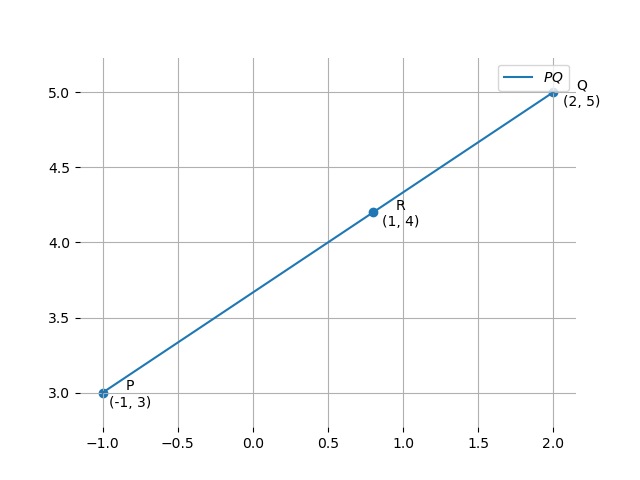
\includegraphics[width=0.7\linewidth]{figs/plot1.png}
\label{fig1}
\end{figure}
\end{document}
